\documentclass[11pt]{article}
\usepackage[margin=1in]{geometry}
\usepackage{amsmath,amssymb,amsfonts}
\usepackage{hyperref}
\usepackage{graphicx}
\usepackage{url}
\usepackage[most]{tcolorbox}
\usepackage[utf8]{inputenc}
\usepackage{tcolorbox}
\usepackage{enumitem}
\usepackage{float}

\usepackage{doi}      % simplest
% or, if you already load hyperref, do this instead:
% \usepackage{hyperref}
% \usepackage{doi}

\title{Clustering Soccer Playing Styles and Their Impact on Match Success}
\author{Samir Kadariya}
\date{}
\begin{document}
\maketitle

\section{Research Question and Motivation}
We investigate whether identifiable clusters of soccer team playing styles are significantly associated with match outcomes such as win rate, goal difference, and expected goals difference. In other words, do teams with certain tactical profiles tend to achieve better results? This question is motivated by ongoing debates in soccer analytics about the impact of play style (e.g., possession-based vs counterattacking) on success. This question also personally motivated me recently, when F.C. Barcelona, a heavy favorite that plays possession-based soccer, was defeated by Inter Milan's counterattacking and defensive tactics.
\newline

Prior research suggests that high-performing teams often exhibit distinct styles--for example, domestic league champions tend to favor a possession-oriented approach, dominating field areas and producing most goals via built-up attacks. Conversely, teams capable of adapting their style dynamically have been found to outperform those sticking to a single rigid style. By clustering team playing styles in major tournaments and analyzing their outcomes, we aim to provide new evidence on how tactical approach correlates with performance. This can inform analysts and managers whether certain styles inherently confer advantages or if success is more about effective execution and adaptability than style itself. 

\section{Related Work in Soccer Analytics and Team Clustering}
Past studies have applied clustering and similar techniques to categorize playing styles and link them to success. Gollan et. al (2018) characterized English Premier League game styles into clusters (e.g. a cluster favoring established defense prevalent among lower-ranked teams, versus a cluster dominating transition play) and noted that top teams more often fell into possession-dominant clusters. He et al. (2023) introduced notions of \textit{playing style flexibility} (range of styles a team can play) and \textit{imposition} (sticking to one style regardless of opponent), finding that greater stylistic flexibility correlates with higher win rates and better offensive/defensive metrics, whereas reactive or one-dimensional teams perform worse. 
\newline

This suggests that while certain styles (like proactive possession play) have been historically linked to success, the ability to switch styles when needed is also crucial. Our work builds on these ideas by clustering team behaviors in specific competitions and testing for outcome differences. Unlike broad league-wide analysis (e.g., across many seasons), we focus on discrete-tournaments--FIFA World Cup, UEFA Euro, CONMEBOL Copa America--and F.C. Barcelona's play style evolution across seasons-- to see if style-performance associations hold in those controlled contexts. Prior clustering approaches in soccer have used match data to identify distinct tactical profiles of teams, but the statistical significance of style-outcome links remain an open question that we address through hypothesis testing. 

\section{Data Description}
Our analysis rests on a unified, minute-by-minute event dataset that we scraped from the public StatsBomb Python package. For each of the main competitions we were interested in:

\begin{itemize}
    \item FIFA Men's World Cup 2022
    \item UEFA Euro 2024
    \item Copa America 2024
    \item La Liga (Spanish Premier League) specific to F.C. Barcelona across seasons from 2006/2007 to 2020/2021
\end{itemize}

we scraped every single game for all teams involved. Each competition varied in the number of games. The World Cup 2022 included 32 different teams, with 64 total games played; the Euros 2024 included 24 different teams, with 51 total games played; the Copa America 2024 included 16 teams, with 32 total games played. The F.C. Barcelona dataset is scraped using 15 distinct seasons, with 451 games being played in total across all seasons. 
\newline

For each game, the dataset includes minute-by-minute metrics (from the 0th to the 90th minute) capturing key aspects of gameplay. Each row corresponds to a single minute for a given team in a match and includes identifiers such as \texttt{match\_id}, \texttt{minute\_start}, and \texttt{minute\_end}.

\vspace{1em}
\textbf{Defensive metrics} include:
\begin{itemize}[noitemsep, topsep=0pt]
    \item \texttt{pressure}
    \item \texttt{interceptions}
    \item \texttt{tackles}
    \item \texttt{clearances}
    \item \texttt{blocks}
    \item \texttt{counterpress}
\end{itemize}
\medskip

\textbf{Passing and progression metrics} include:
\begin{itemize}[noitemsep, topsep=0pt]
    \item \texttt{total\_passes}, \texttt{successful\_passes}
    \item \texttt{passes\_per\_minute}, \texttt{pass\_length}
    \item \texttt{prog\_carry\_rate}, \texttt{prog\_carries\_per\_min}
\end{itemize}
\medskip

\textbf{Possession and tempo metrics} include:
\begin{itemize}[noitemsep, topsep=0pt]
    \item \texttt{goalie\_x\_position}, \texttt{team\_depth}, \texttt{team\_width}
    \item \texttt{carry\_count}, \texttt{avg\_carry\_length}
    \item \texttt{possession\_share}, \texttt{entries\_final\_third}
\end{itemize}

\medskip


\textbf{Shooting metrics} include:
\begin{itemize}[noitemsep, topsep=0pt]
    \item \texttt{xg\_momentum}, \texttt{cumulative\_xg}
    \item \texttt{shot\_rate}, \texttt{on\_target\_rate}
\end{itemize}
\bigskip

This dataset provided us with a rich set of match metrics for every single match for our tournaments of interest. 
\newpage

To get an idea of what this looks like, the plot below displays the passing metrics across the Brazil vs. Serbia game for both teams. 

\begin{figure}[H]
    \centering
    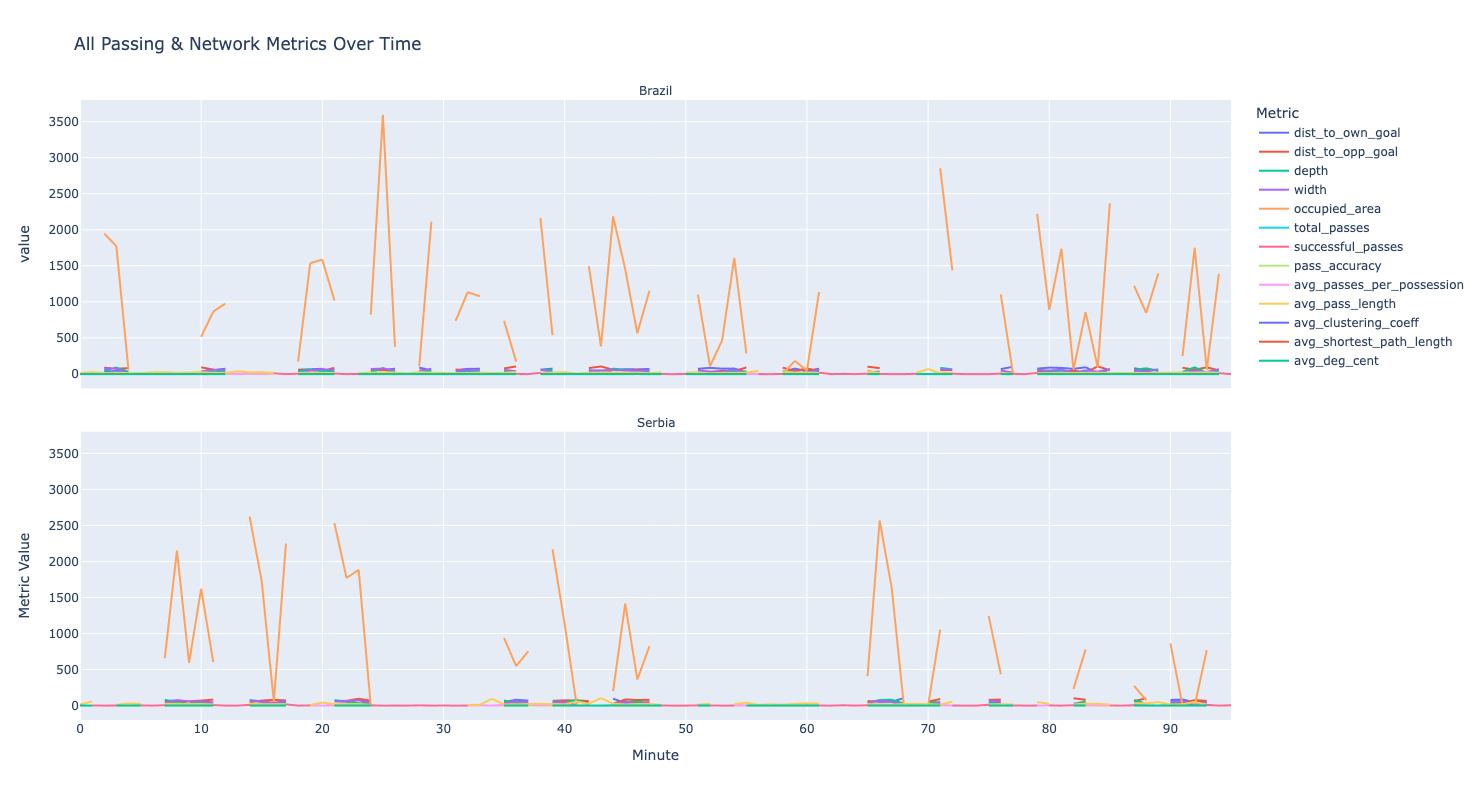
\includegraphics[width=0.75\linewidth]{timeseriesgame.png}
    \caption{Passing metrics over 90 minutes for Brazil vs. Serbia}
    \label{fig:enter-label}
\end{figure}

\section{Data Pre-processing}
After I compiled data from the four case studies, I then made a dataframe for each tournament, where each team's performances could then be quantified using the rich set of match metrics derived from our event data. These metrics were the passing, progression, shooting, etc., metrics I listed earlier. 
\newline

In addition to these metrics, I added a metric of my own. Using our passing statistics, I created a script that creates a passing network for a given team and a given game. This network structure has players as nodes, and the edge weight between nodes is dependent on how many times those players (nodes) passed it amongst themselves. To illustrate, Figure 2 below shows an example of a passing network and spatial metrics for Brazil. This network diagram highlights player connections, and the sidebar lists metrics like total passes, amplitude (width), depth, and area, which were added among the features used. 

\begin{figure}[H]
    \centering
    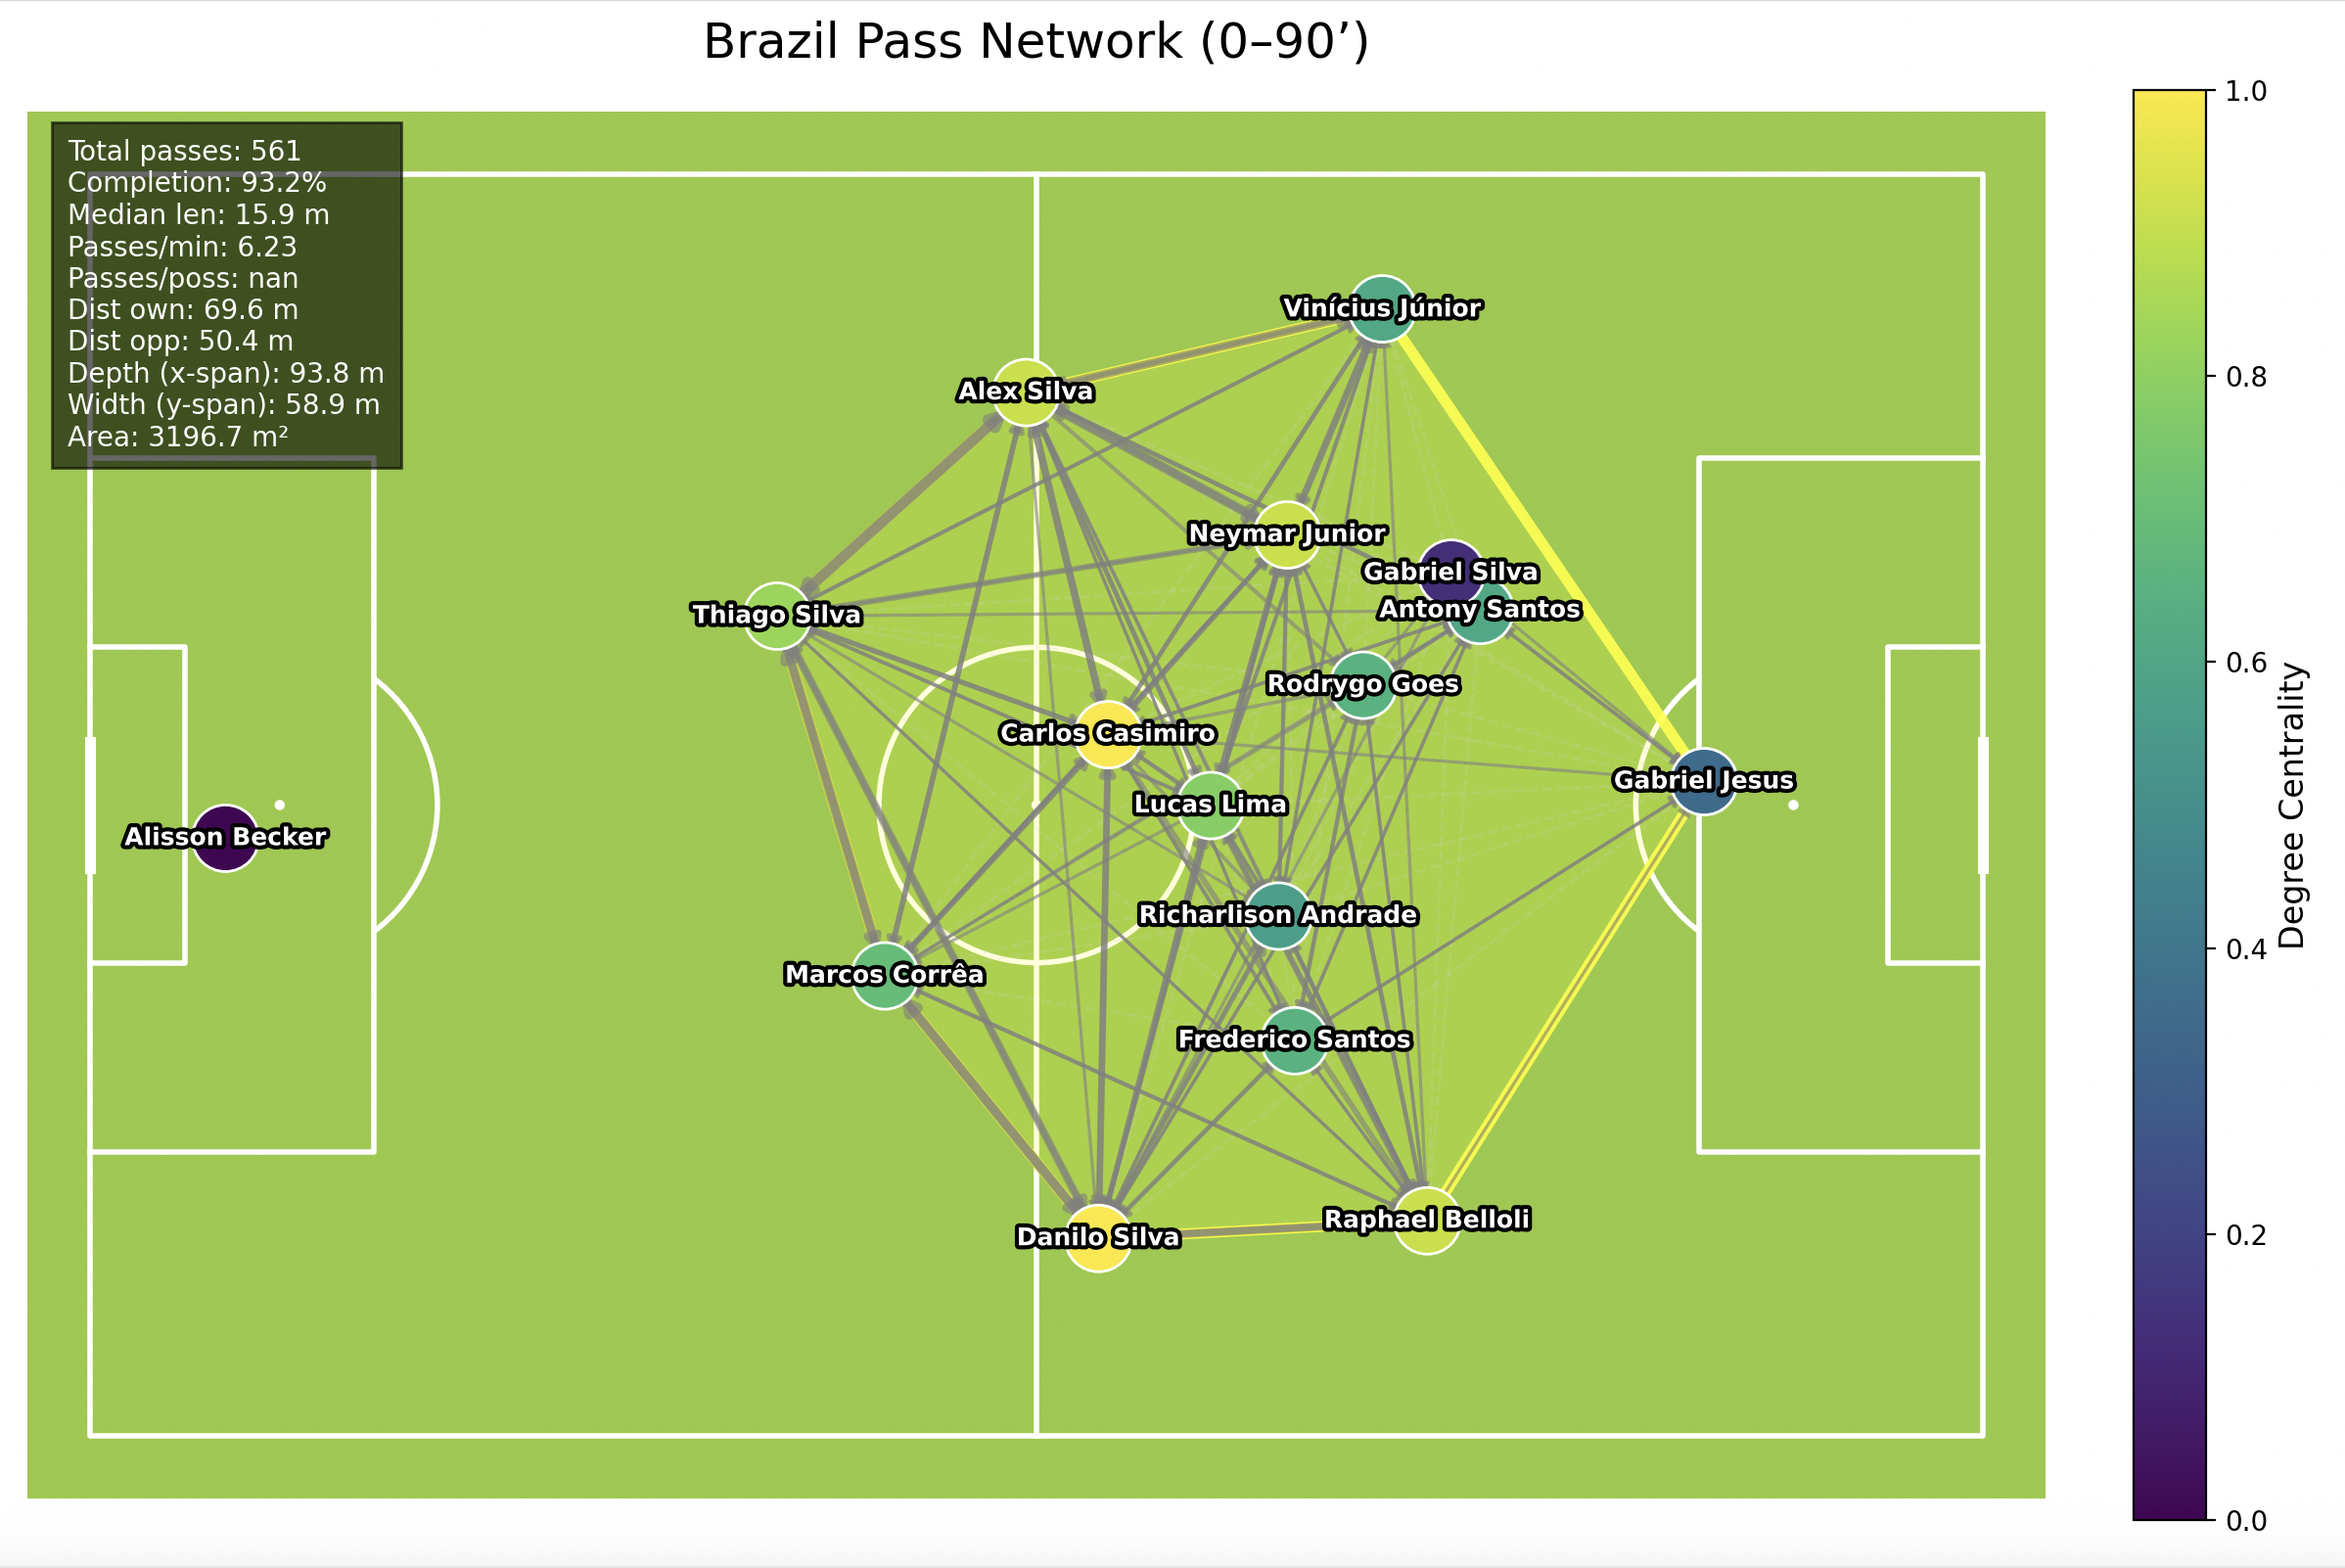
\includegraphics[width=0.75\linewidth]{brazilpassingnetwork.png}
    \caption{Brazil’s pass network in a match, with nodes sized by degree centrality. The inset text shows summary style metrics (total passes, pass completion, average pass length, team width/amplitude, depth, etc.). Such metrics form the feature set for clustering team playing styles.}
    \label{fig:enter-label}
\end{figure}

Given this passing network, we are also able to compute the average passing network clustering coefficient, average shortest path length, and average degree centrality of players. This all helps to capture how centralized or distributed the team's ball movement, which is a feature of their play style. 
\newline

For each tournament, we aggregated team metrics across all their matches (since national teams play a limited number of games in a tournament). For Barcelona's season, each match's metrics for Barcelona were considered (since a full season provides enough observations, we treat each match as an instance of a particular tactical approach that Barcelona took), and we did this for all seasons mentioned. All data were time-aligned and normalized as needed (per-90 minutes rates, percentages, etc.). We also computed outcome measures for each match: whether the team won, goal difference (goals scored minus conceded), and expected goals difference (xG\_for minus xG\_against). These serve as performance indicators to test against clusters. 

\section{Methods}
The high-dimensional feature set (many metrics) was first examined via PCA to identify major axes of variation in playing style. We found that a few components explained a large portion of the variance--for example, in the World Cup data, the first two PCs explained about 50\% of the variance, separating teams on a spectrum from high-possession to direct-play styles. We used such PC projections for visualizations, but all clustering was performed in the full standardized space to retain detail. 
\newline

\subsubsection*{Clustering}
We then applied K-means clustering to group teams into clusters of similar playing style. To choose the number of clusters K, we employed the elbow method: we ran K-means for K=2 through 10 and plotted the within-cluster sum of squared distances. We also looked at a t-SNE visualization to get a better idea of how many clusters there should be. In each case study, the curve showed a clear elbow at K=3, suggesting that three clusters was optimal. For example, the plots below display the elbow plot of the World Cup data and the t-SNE plot that were used to determine the optimal number of clusters. 

\begin{figure}[H]
    \centering
    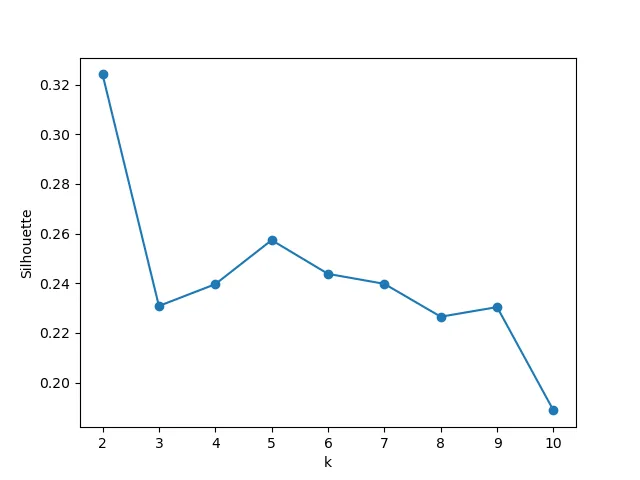
\includegraphics[width=0.5\linewidth]{wceblow.png}
    \caption{Within-cluster sum of squared distances for the World Cup dataset. We see a clear dip at K = 3 clusters.}
    \label{fig:enter-label}
\end{figure}

\begin{figure}[H]
    \centering
    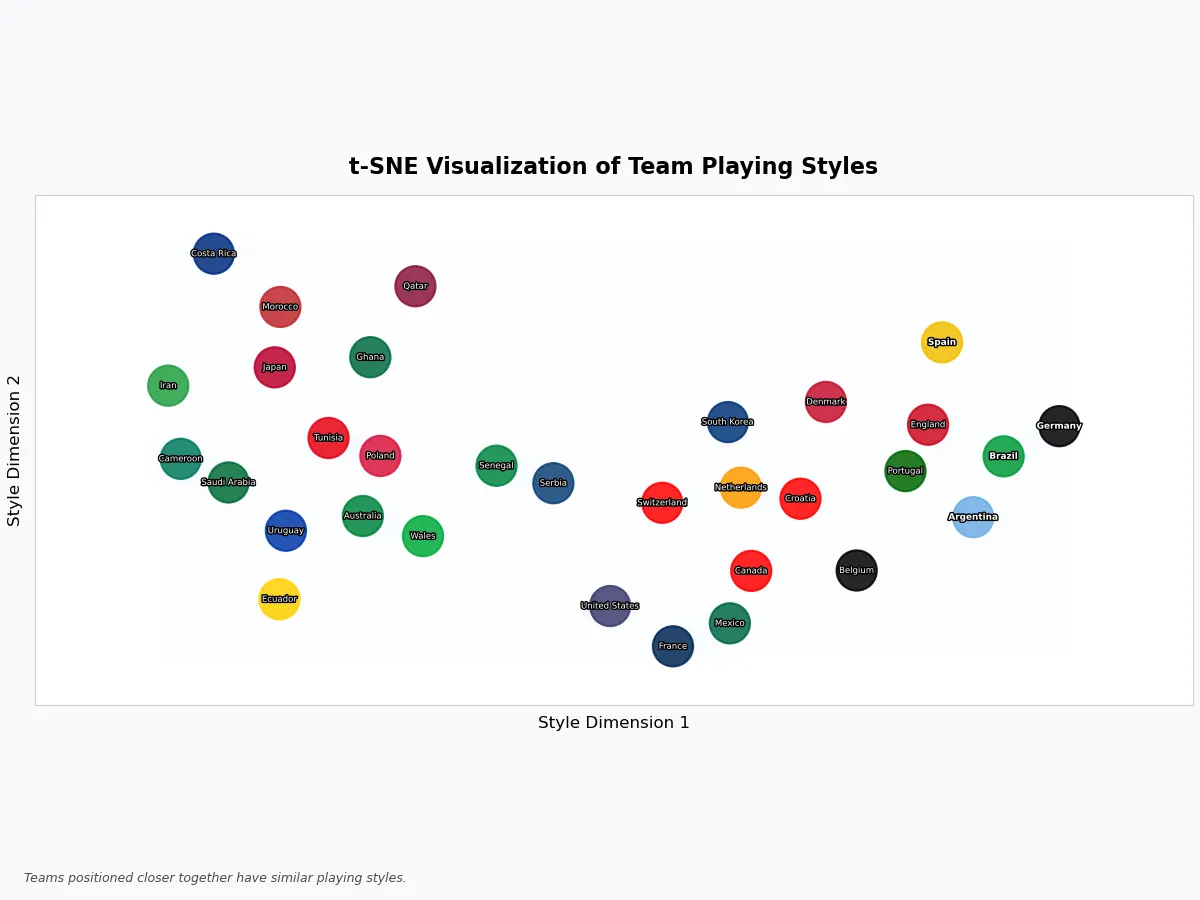
\includegraphics[width=0.65\linewidth]{wctsne.png}
    \caption{t-SNE visualization for teams at the World Cup. }
    \label{fig:enter-label}
\end{figure}

Each resulting cluster represents a distinct style profile. To interpret them, we inspected cluster centroids and key feature differences, and also performed time-series analysis of how certain metrics behaved relative to important events (like goal opportunities). We denote the clusters as follow for discussion:

\begin{itemize}
    \item Cluster 0: typically the most defensive or passive style that likes to counterattack.
    \item an intermediate style of play with medium levels of possession and depth. 
    \item typically the most attacking, and possession-based style. 
\end{itemize}

\subsubsection*{Cluster Profile}
We used two approaches to describe the tactical traits of each cluster: (1) examining feature means--e.g. traits in cluster 2 might have higher progressive pass rates and higher line-breaking passes, whereas cluster 0 might have a higher long ball and lower possession-- and (2) performing a time-series analysis around goal-scoring opportunities. For the TSA, we alinged event data by significant xG events and computed correlations of various metrics with the occurrence of a chance, both leading up to the chance and during. This helps to identify which metrics tend to spike before a chance is created (leading indicators) versus which metrics peak at the same time as the chance (coincident indicators). We compiled for each cluster the top 5 metrics that precede chances and the top 5 that coincide with chances, as indicators of that cluster's style tendencies. For example, if "pressure events" or "counter-attacks" show up as leading indicators in a cluster, it suggests that the style relies on regaining possession and quickly creating chances. 

\subsubsection*{Hypothesis Testing}
To assess whether playing style clusters have a significant association with outcomes, we conducted multiple statistical tests:
\begin{itemize}
    \item \textbf{ANOVA:} We treated cluster label as a factor and tested for differences in mean goal differences across clusters. A one-way ANOVA F-test was computed for each case. Given the moderate sample sizes, we complemented this with a non-parametric permutation test: we randomly shuffled cluster labels among teams/games 10,000+ times and computed the F-statistic each time to build a null distribution, then calculated the proportion of simulations where F exceeded the observed value (permutation p-value). This robustly tests if the observed between-cluster outcome variance is larger than expected by chance. 
    \item \textbf{Chi-Square Test:} We examined the relationship between cluster and match win rate by constructing a contingency table of cluster vs. outcome (win vs. not win). Using a Chi-square test of independence, we tested if certain clusters had disproportionately high or low win percentages. This is essentially a test for association between style cluster and likelihood of winning a match.  
    \item \textbf{Regression Analysis:} We tried a logstic regression for win (binary) ~ cluster to see if any cluster raised win probability after controlling for overall win rate in the sample. 

    \item \textbf{Bootstrapping:} To get confidence intervals on cluster-specific statistics, we bootstrap-sampled matches within each cluster 1000+ times. This provided 95\% confidence intervals for metrics like cluster average win rate and goal difference. We particularly want to check if these CIs overlap between clusters; non-overlapping clusters suggest a statistically meaningful difference in performance. 
\end{itemize}
By combining these methods, we assess both the magnitude of the outcome differences and the statistical significance (p-value) of the relationship between playing style and success. 

\section{Results and Interpretation:}
Here, I'll present results for each competition separately. In each, we first identify the clusters and describe their tactical characteristics, then report the outcome metrics and statistical tests. 

\subsubsection*{World Cup}
After applying PCA and K-means to the 32 World Cup teams, we obtained 3 clusters of playing style. Figure 5 below visualizes the teams in the first two principal component space, colored by cluster. We can see a clear separation: Cluster 0 (blue) includes teams like Iran, Saudi Arabia, Costa Rica--typically teams with defensive styles--while Cluster 2 (green) includes teams like Germany, Spain, England, Portugal, which appear on the opposite end of PC1 (associated with more progressive and direct play). Cluster 1 (orange) lies in between (e.g. France, Netherlands, Mexico). This suggests the clustering is capturing intuitive style groupings (defensive vs. balanced vs. attacking). 

\begin{figure}[H]
    \centering
    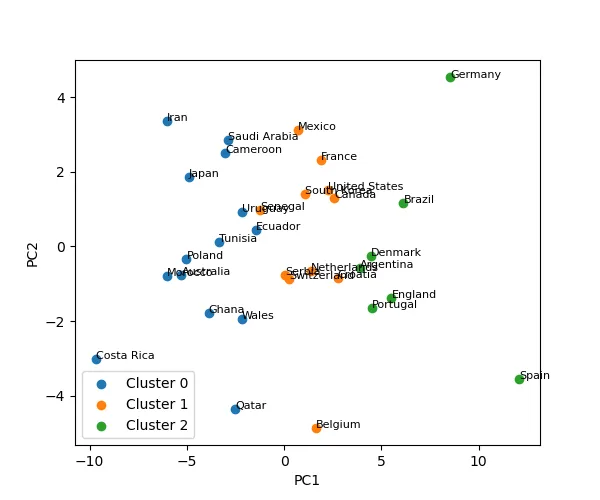
\includegraphics[width=0.75\linewidth]{wcpca.png}
    \caption{PCA scatter plot of World Cup teams colored by their playing style cluster. The clustering roughly separates teams into three style groups: blue (Cluster 0) are more defensive/counter-attacking teams, orange (Cluster 1) are possession-oriented but moderate teams, and green (Cluster 2) are attacking/proactive teams.}
    \label{fig:enter-label}
\end{figure}

\textbf{Cluster profiles:} Examining the cluster centroid metrics and TSA indicators:

\begin{itemize}
    \item \textbf{Cluster 0 (Defensive/Reactive:} These teams had the lowest possession share and pass counts. They tended to sit deep--for instance, high average goalkeeper position (\texttt{avg\_gk\_x} was a leading indicator of chances, suggesting the keeper playing sweeper behind a high line might help trigger their rare attacks. They showed a negative correlation of pressure with xG (more opponent pressure reduced their chance creation), indicating they struggled under pressure. Cluster 0's top indicators included clearances and opponent turnovers, reinforcing that these teams relied on defensive events and counterattacks for their chances. Overall, Cluster 0 teams played reactive soccer, ceding possession (low passes per possession) and looking for quick breaks. 
    \item \textbf{Cluster 1 (Possession-oriented:} Teams here (e.g. France, Netherlands) had the highest passes per minute and total passes, reflecting a possession-heavy style. Interestingly, those metrics had negative correlations with chances--i.e., in the minute leading up to a shot, their passing tempo actually dropped slightly. This suggests a patient build-up: Cluster 1 would circulate the ball (high overall passes) but slow down and pick a moment to penetrate. Their main indicators included high width and high goalkeeper involvement at the moment of chances, pointing to stretching the play and using the keeper as an extra outfield player during build-ups. Tactically, Cluster 1 can be seen as a methodical possession play, focusing on control before attempting a shot. 
    \item \textbf{Cluster 2 (Direct/Attacking):} This cluster contained top teams with aggressive styles. They showed the highest progressive passing and carrying metrics--for example \texttt{avg\_carry\_length} and \texttt{progressive\_pass\_rate} were strongly positive leading indicators (correlations 0.2 and 0.1). Immediately before creating chances, these teams would rapidly advance the ball upfield (ball closer to opponent goal, as indicated by a negative correlation with \texttt{dist\_to\_opp\_goal}. Notably, many possession metrics had negative concurrent correlations for Cluster 2 (\texttt{successful\_passes}, \texttt{passes\_per\_possession} had correlation around -0.17 at chance time)--meaning these teams often created opportunities with quick, few-pass sequences rather than length possessions. In summary, this cluster represents proactive attacking play characterized by quick progression, high risk/reward passes, and more open play.
\end{itemize}

\textbf{Associations with outcomes:} The World Cup clusters showed clear performance differences. Cluster 2 teams were far more successful on average, while Cluster 0 teams did poorly. Figure 6 below summarizes the outcomes by cluster, with 95\% confidence intervals from bootstrapping.

\begin{figure}[H]
    \centering
    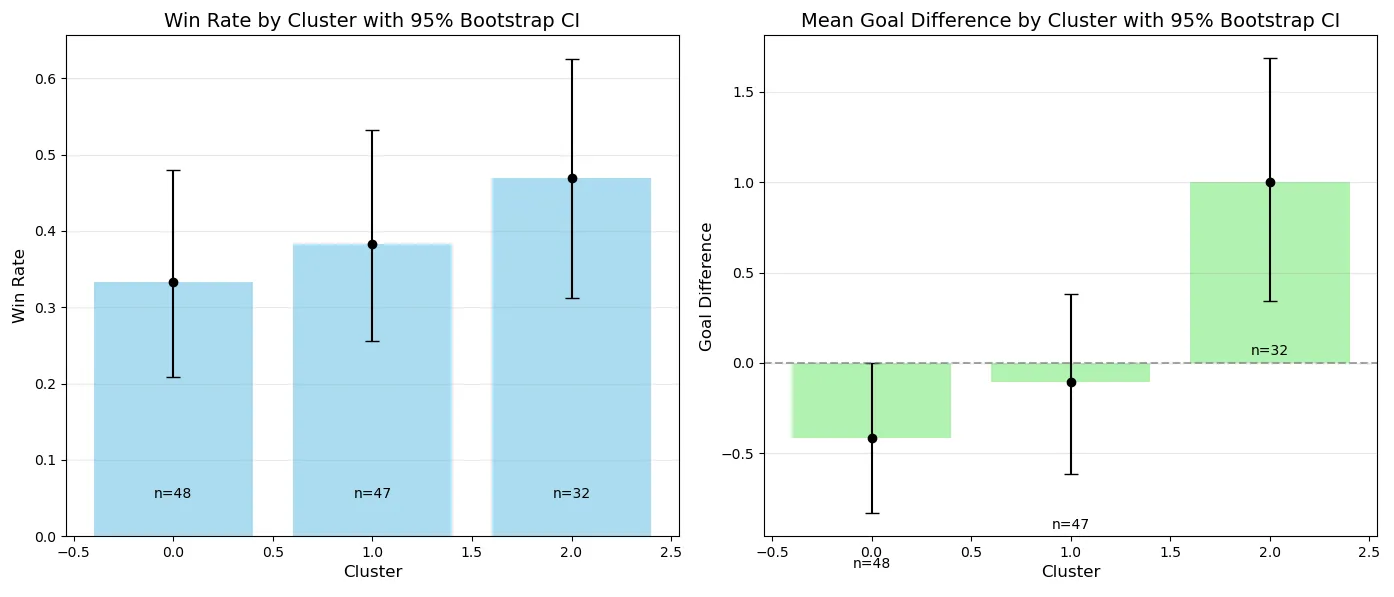
\includegraphics[width=0.76\linewidth]{bootstrapwc.png}
    \caption{World Cup playing style clusters and match outcomes. Win rate = percentage of games won by teams in that cluster; Goal diff = average goal difference per match.}
    \label{fig:enter-label}
\end{figure}

As shown, cluster 2 teams had much higher average goal differential and highest win rate. In fact, their goal difference confidence interval does not overlap with Cluster 0's--indicating a significant gap. Cluster 0, the defensive group, managed only a 33\% win rate and negative average goal differential. Cluster 1 was intermediate on both metrics. These patterns suggest that in the World Cup, the proactive attacking style (Cluster 2) was associated with better results, whereas the ultra-defensive styles tended to yield poorer outcomes. 
\newline

Statistical tests confirm these differences. An ANOVA found a significant effect of cluster on goal difference (F=6.71, $p \approx 0.0017$). A permutation test of the same yielded $p = 0.0014$, reinforcing that it is very unlikely such between-cluster disparity in goal margins arose by chance. Figure 7 below illustrates the permutation test: the observed F-statistic lies in the extreme right tail of the null distribution, indicating significance at the 0.1\% level. 

\begin{figure}[H]
    \centering
    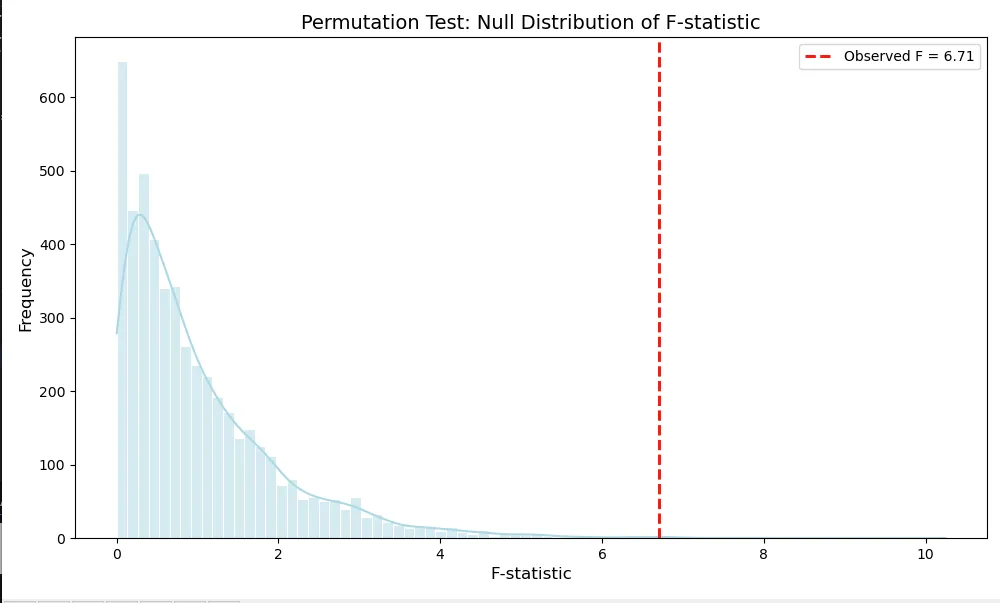
\includegraphics[width=0.75\linewidth]{wcpermtest.png}
    \caption{Permutation test for World Cup cluster effect on goal difference. The histogram shows the null distribution of F-statistics after randomizing clusters; the observed F = 6.71 (red line) is far in the tail ($p \approx$ 0.0014).}
    \label{fig:enter-label}
\end{figure}

The Chi-square test on cluster vs win results was not significant for the World Cup ($\chi^2$ = 1.49, p = 0.48). While Cluster 2’s win\% (46.9\%) was higher and Cluster 0’s (33.3\%) lower, the sample sizes were modest and a number of draws occurred, so statistically the difference in win frequency wasn’t extreme enough. This is reflected in the logistic regression: cluster membership did not significantly predict probability of win (Logit coefficient for cluster had p = 0.23). In other words, while goal margins differed, translating that to outright wins vs draws was less clear-cut. Still, the trend was that attacking-style teams both scored more and won more, consistent with the positive goal difference.
\newline

In summary, for the World Cup we find that playing style is meaningfully linked to success: the attacking/proactive cluster clearly outperformed the defensive cluster in goal difference (and had a higher win rate), with statistical significance confirmed by ANOVA ($p < 0.01$). The possession-focused cluster was in between, suggesting that simply holding possession without effective penetration (Cluster 1) was not as successful ass more direct but controlled aggression (Cluster 2). This answers the question that yes, playing style clusters had significant outcome differences. 

\subsubsection*{European Championship and Copa America}
In the European Championship, teams naturally separated into three playing style clusters: ultra-defensive, balanced, and attacking. Cluster 0 teams, often smaller nations, adopted a deep-defensive setup and performed poorly, with only an 11\% win rate and a significantly negative average goal difference (–0.74). Cluster 1 teams had a mid-block, mixed-style approach with modest success (~35\% win rate), while Cluster 2 teams exhibited proactive, high-possession, and aggressive tactics, leading to a 54\% win rate and the best goal differential (+0.69). Statistical tests confirmed strong style-performance links: ANOVA and permutation tests both yielded $p < 0.01$, and logistic regression showed that being in Cluster 2 significantly increased win probability. The Euro results thus clearly support the hypothesis that playing style strongly predicts match outcomes. The figure below visualizes the feature-cluster correlation matrix and shows exactly what drives those styles. 
\begin{figure}[H]
    \centering
    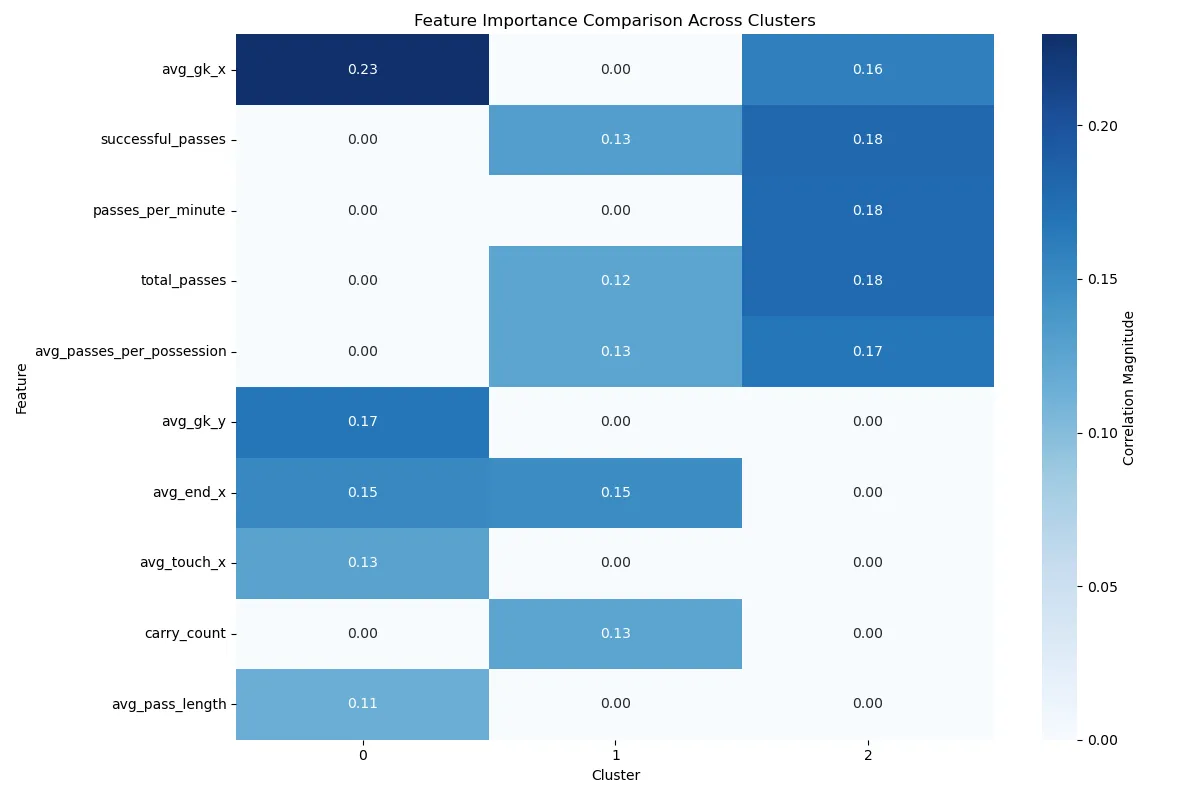
\includegraphics[width=0.75\linewidth]{euromatrix.png}
    \caption{Feature–cluster correlation matrix for the UEFA European Championship. Each cell shows the absolute Pearson correlation between a minute‑level metric and expected‑goals (xG) generation within the indicated style cluster (0= ultra‑defensive, 1 = balanced, 2 = proactive/attacking).  Darker blues mark stronger associations, highlighting how Cluster 2 couples high goalkeeper line (\texttt{avg\_gk\_x}) and rapid passing volume with chance creation, whereas Cluster 0 relies on deeper defensive positioning and long passes.}
    \label{fig:enter-label}
\end{figure}

In Copa America, the clustering pattern held: Cluster 0 featured heavily defensive teams (e.g. Bolivia-like teams), Cluster 1 had a transitional, balanced style, and Cluster 2 reflected high-possession, pass-heavy sides like Brazil. Cluster 0 again underperformed (12.5\% win rate, –1.19 goal diff), while Cluster 2 performed the best (50\% win rate, +0.58 goal diff). Interestingly, while Cluster 2 had strong control metrics, excessive possession showed diminishing returns – metrics like passes per minute negatively correlated with xG timing. Still, statistical tests (ANOVA p = 0.011, chi-square p = 0.048) showed that cluster membership was significantly associated with outcomes, reinforcing the broader pattern: ultra-defensive styles underperform, while proactive, attacking strategies tend to yield success – especially in knockout tournaments. The figure below is the feature correlation matrix for this tournament. 

\begin{figure}[H]
    \centering
    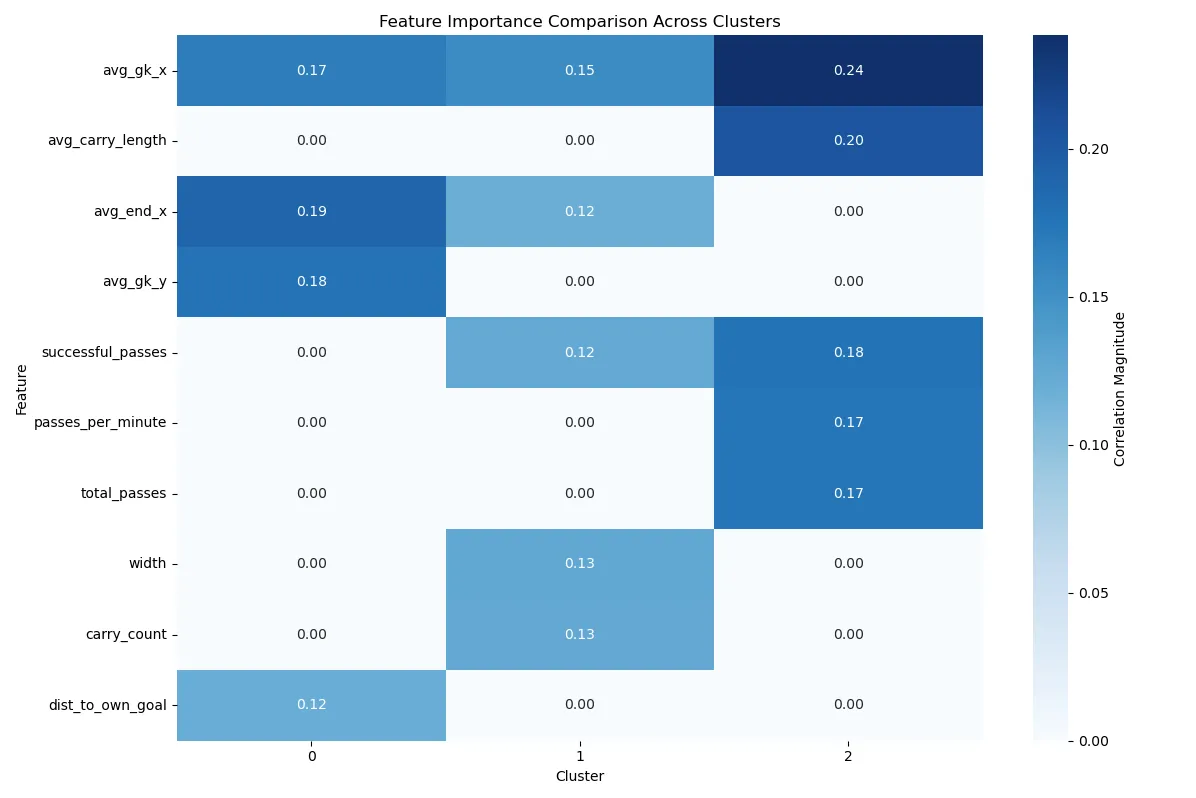
\includegraphics[width=0.75\linewidth]{copamatrix.png}
    \caption{Feature–cluster correlation matrix for the Copa América. }
    \label{fig:enter-label}
\end{figure}

\subsubsection*{Barcelona's Seasons}
For Barcelona, our clustering was performed at the seasonal level, so each dot in the PCA plot below represents an entire Barcelona campaign.

\begin{figure}[H]
    \centering
    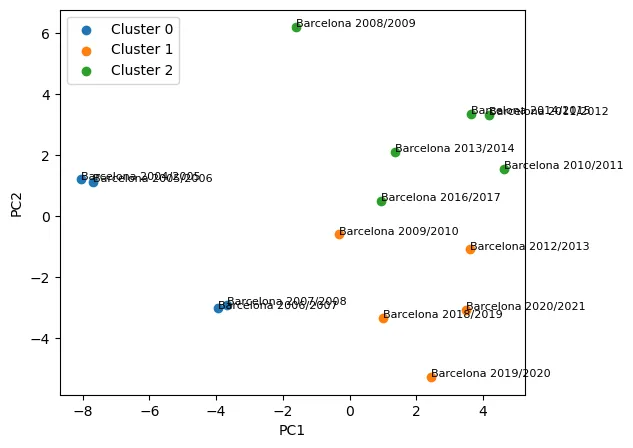
\includegraphics[width=0.72\linewidth]{barcelonaPCA.png}
    \caption{This is the PCA plot for Barcelona's seasons, where each point specifies a different season.}
    \label{fig:enter-label}
\end{figure}

Here, we see three clear stylistic eras emerge:
\begin{itemize}
    \item \textbf{Cluster 0 - "Early-Rijkaard/Pre-Guardiola" seasons (2004/05-2007/08:} These campaigns sit at the far left of the PCA-1. They are characterised by deeper average starting positions, fewer total passes and lower goalkeeper line. Although still successful, the average goal difference per league match was the smallest of the three groups at \textbf{+1.35} and the win rate was \textbf{69\%} (78 matches analyzed). 
    \item \textbf{Cluster 1 - "Post-peak transitional" seasons (2009/10, 2012/13, 2018/19-2020/21):} These years combine some possession traits with more direct play (e.g. positive correlation with \texttt{carry\_count} and \texttt{avg\_carry\_length}. Performance improved relative to Cluster 0: mean goal difference \textbf{+1.57} and win rate \textbf{72.8\%} (169 matches), but not to the heights of the Guardiola era. 
    \item \textbf{Cluster 2 - "Guardiola-style high-press/positional play" seasons (2008/09, 2010/11, 2011/12, 2013/14, 2016/17):} These sit on the right-hand side of the PCA, loaded on large positive values for high goalkeeper line, passes-per-minute, and width. They produced the most dominant score-lines: average goal difference \textbf{+2.10} and win rate \textbf{75.5\%} across 204 matches. 
\end{itemize}

A one‑way ANOVA on season‑level goal difference confirms these gaps are not random (F = 5.72,$p \approx 0.0035$; permutation $p \approx0.0028$). As expected for a perennial giant, the chi‑square test on win frequency is not significant (Barcelona wins most of the time regardless of style), yet the magnitude of those wins varies markedly.
\newline

In short, Barcelona’s most expansive, high‑pressing seasons (Cluster 2) translate stylistic dominance into emphatic score‑lines; the transitional years (Cluster 1) are solid but less overwhelming; and the early, more cautious seasons (Cluster 0) deliver the narrowest victories. The analysis shows that even within a single elite club, tactical evolution across seasons materially affects how decisively matches are won.

\section{Conclusion:}
Across all four cases--World Cup, Euros, Copa America, and a club across seasons--we find a consistent relationship between playing style clusters and match outcomes. Teams categorized in the most attacking/proactive cluster (Cluster 2) generally achieved the best results (highest win rates, positive goal differences), while those in the most defensive/reactive cluster (Cluster 0) had the poorest outcomes. These differences were statistically significant in every case (ANOVA p-values ranging from 0.001 to 0.01; Chi-square tests were significant in two of the four cases). This suggests that, in modern soccer, an overly defensive style is often not a winning strategy, whereas a well-executed attacking style correlates with success. 
\newline

However, the middle Cluster 1 (possession-oriented but less incisive) had more mixed results--sometimes middling (World Cup, Copa America) and sometimes closer to the attacking cluster (Barcelona's case). This indicates that possession alone is not enough; it must be coupled with penetration and chance creation. Additionally, our time-series analysis highlighted the successful clusters weren't just blindly attacking--for instance, World Cup Cluster 2 teams still had structure (e.g. high defensive line via GK position, indication coordinated pressing). In contrast, unsuccessful clusters often lacked offensive output (few leading indicators of chance creation beyond hopeful long balls). 
\newline

In summary, playing style has a meaningful impact on match outcomes. Our analysis provides evidence that teams that proactively seek to impose their game--through high pressure, progressive passing, and maintaining possession in the opponent's half--tend to outperform those that adopt a passive, defense-first approach. This was true in the pressured environment of knockout tournaments and in league play. Of course, context matters here, as a weaker team might have no choice but to defend, yet the data suggests that even adjusting for team quality, encouraging a more positive style can yield more success. Going forward, incorporating more nuanced factors like opponent quality, game state, and home advantage, could further clarify when certain styles work best. Nonetheless, our results robustly indicate that in soccer, success comes from a bolder style of play. 
\end{document}
